\subsection{Begriffe und Definitionen}
\label{sub:begriffe}
  Bevor im nächsten Kapitel "`\nameref{sec:develop}"' die Umsetzung des Projekts beschriebene wird, sollen zuerst die Begrifflichkeiten und Definitionen festgelegt werden, um ein einheitliches Verständnis zu garantieren.

  \subsubsection{Time}
  \label{ssub:time}
    In verschiedenen Formeln wird immer wieder eine Time $t_{cur}$ referenziert. Diese beschreibt die Globale (aktuelle) Zeit des Systems in Sekunden. 
    Die Sekunden lassen sich durch das Addieren der Stunden, Minuten und Sekunden errechnen.\\

    Bsp: 17:04:59 Uhr\\

    $t_{cur} = $ Stunden $*$ 3600 $+$ Minuten $*$ 60 $+$ Sekunden\\
    $\Rightarrow$ $t_{cur} = 17 * 3600 + 4 * 60 + 59 = 61499 \; sec$
    
  % subsubsection time (end)

  \subsubsection{Vehicle}
  \label{ssub:vehicle}
    Ein Vehicle $V$ beschreibt in dieser Arbeit ein Fahrzeug, welches im Dienste der öffentlichen Verkehrsbeförderung steht. Beispielsweise Bus, U- \& S-Bahn, Interrail Züge aber auch Zahnradbahn oder gar Funicular-Services\footnote{\url{https://en.wikipedia.org/wiki/Funicular}}. Das private Automobil fällt folglich nicht unter diese Definition.
  % subsubsection vehicle (end)

  \subsubsection{Polyline}
  \label{ssub:polyline}
    Eine Polyline\footnote{Linienverlauf bzw auch Shape genannt} $P$ ist eine Kurve die sich durch eine Sequenz an Punkten $\{ p_1, \dotsc, p_n \;|\; n \in \mathbb{N} \}$ definiert. Sie beschreibt den zurückzulegenden Verlauf eines Vehicles.
  % subsubsection polyline (end)

  \subsubsection{Station}
  \label{ssub:station}
    Eine Station $S$ ist eine Haltestelle, die von einem Vehicle $V$ während eines Trips $T$ angefahren wird und sich entlang einer Polyline befindet. Die Station definiert dabei die Ankunfts- und Abfahrtszeiten, wann ein Vehicle an dieser Station anhaltet und wann es diese zur Weiterfahrt wieder verlässt. Ankunfts- und Abfahrtszeit seien wie folgt definiert: \texttt{arrival time} $ := t_{ari}$ und \texttt{departure time} $ := t_{dep}$.

  \subsubsection{Trip}
  \label{ssub:trip}
    In dieser Arbeit wird immer wieder der Begriff "`Trip"' Verwendung finden. Ein Trip $T$ sei mit folgenden Eigenschaften definiert:
    \begin{itemize}
      \item $T$ besteht aus einer Anzahl an Stationen: $T = \{S_1, \dotsc, S_n \;|\; n \in \mathbb{N}, n \geq 2 \}$

      \item Ein Trip $T$ wird dabei von genau einem Vehicle $V$ bedient. Daraus folgt $T$ mit dem Mapping: $T \mapsto V$ ist Injektiv zu $V$. 

      \item Ein Trip $T$ besitzt genau eine Polyline $P$. $T \mapsto P$ $ \Rightarrow T$ ist Injektiv zu $P$. 

      \item Die Bewältigung der Strecke $\{A,B \;|\; A, B \in S\}$ entlang einer Polyline $P$ durch ein Vehicle $V$ gilt als ein einziger Trip.

      \item Ein Trip beginnt genau dann, wenn die momentane Zeit $t_{cur}$ mit der Abfahrtszeit $t_{dep}$ der ersten Station übereinstimmen $\Rightarrow t_{cur} = t_{dep} $ .

      \item Ein Trip endet genau dann, wenn die momentane Zeit $t_{cur}$ mit der Ankunftszeit $t_{ari}$ der letzten Station übereinstimmen $\Rightarrow t_{cur} = t_{ari} $ .

      \item Der Rückweg $\{B, A \ni T \;|\; A, B \in S\}$ ist nicht in einem Trip $T$ enthalten, sondern wird als ein neuer Trip erfasst.
    \end{itemize}
    
  % subsubsection trip (end)

    \subsubsection{Route}
    \label{ssub:route}
      Eine Route $R$ besteht aus einer Anzahl an Trips $T \geq 1$. Eine Route vereint alle vorherigen Relationen in sich. Abbildung \ref{fig:gtfs_viz} veranschaulicht diese. 

      \begin{itemize}
        \item $R = \{ T_1, \dotsc, T_n \;|\; n \in \mathbb{N}, n \geq 1 \}$

        \item $R$ mit dem Mapping: $R \mapsto T$ ist Surjektiv\footnote{Eine Route kann mehrere Trips besitzen, wohingegen ein Trip nur einer Route zugehörig sein kann} 
      \end{itemize}     

      \begin{figure}[htbp]
        \begin{center}
          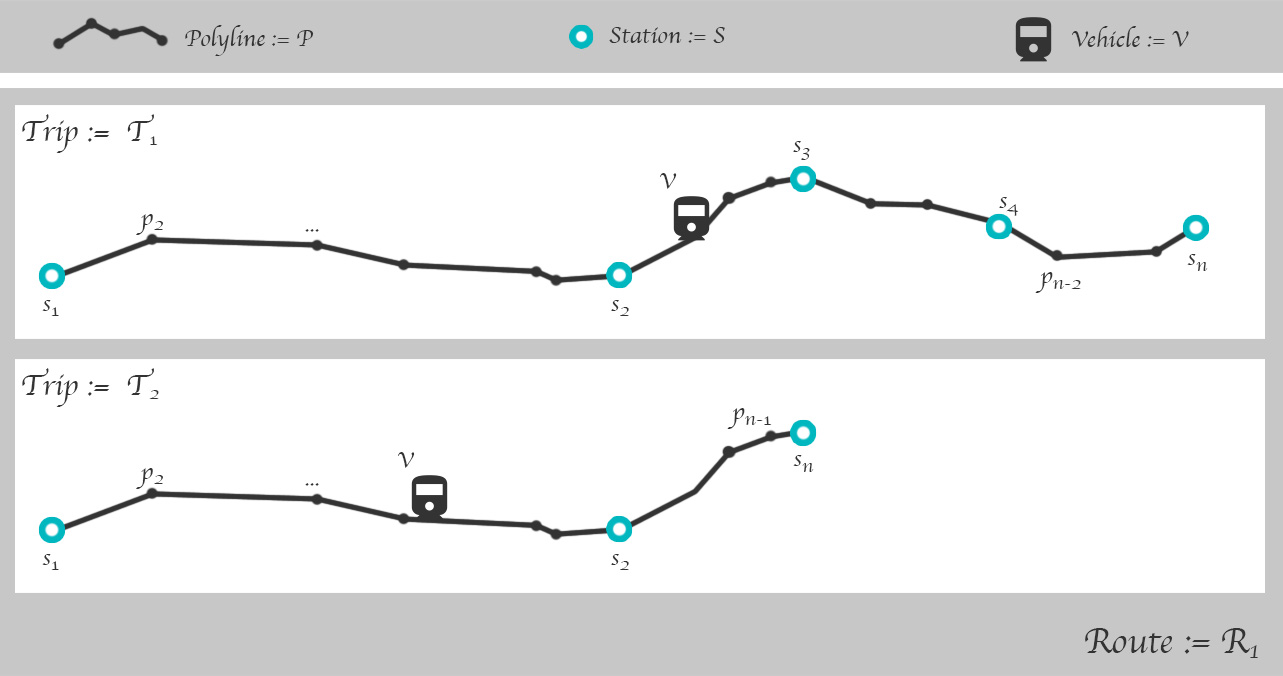
\includegraphics[width=\textwidth]{gtfs_viz.jpg}
          \caption{Grafische Veranschaulichung einer Route}
          \label{fig:gtfs_viz}
        \end{center}
      \end{figure}

      Die Grafik zeigt, dass eine Route zum Beispiel alle Trips einer U-Bahn Linie erfasst. Eine U-Bahn Linie muss dabei nicht immer an allen Stationen halten, sondern kann beispielsweise im Nachtbetrieb auch Stationen auslassen (zu sehen bei Trip $T_2$). Trotzdem werden nur diejenigen Trips in einer Route vereint, die dem selben Routenverlauf folgen.
    % subsubsection route (end)

% subsection begriffe (end)